\chapter{绪\hspace{6pt}论}



\section{研究工作的背景与意义}

随着信息技术的迅猛发展,传统DRAM技术与新兴应用需求之间的矛盾日益突出。在工艺技术层面,DRAM面临着严峻的物理局限性挑战。研究\citing{mutlu2013memory,7838026}指出,当制程工艺迈向10nm及更先进节点时,DRAM存储单元的微缩已逼近物理极限,位密度提升速率显著降低。为维持性能增长趋势,产业界不得不采用多重曝光和极紫外光刻等高复杂度制造工艺,这导致了单位存储容量的制造成本呈指数级上升。根据Patel等人\citing{patel2023xfm}的实证研究,内存系统支出已占据现代数据中心总运营成本的50\%以上,在一些大型互联网公司,这一比例甚至更高,也因此成为制约大规模计算设施扩展的关键瓶颈。此外,DRAM的周期性刷新操作所需能耗随存储容量的增长而显著攀升,这进一步加剧了计算系统的能源效率问题。

与DRAM技术发展面临瓶颈形成鲜明对比的是,现代计算范式对内存系统提出了更为严苛的需求。
当前工作负载如太字节级机器学习\citing{abadi2016tensorflow,lin2012large,rajbhandari2021zero}、大规模图处理\citing{gonzalez2014graphx,sakr2021future}、内存数据库\citing{fitzpatrick2004distributed,Stonebraker2013TheVM}以及其他内存密集型应用程序\citing{atikoglu2012workload,9242282},这一挑战在今天变得更为关键。


然而,实际生产环境中的内存利用状况却不容乐观。Reiss等人\citing{reiss2012heterogeneity}对大规模生产集群的统计分析显示,在70\%的运行时间内,集群平均有30\%的内存处于闲置状态;而在已分配的内存中,实际使用率仅为50\%。这种高成本,低利用率的现象主要由以下因素导致:首先,现代数据中心需要同时支持在线服务、批处理任务、数据分析等多种类型的工作负载,其资源需求和运行时长存在显著差异,导致资源分配难以优化;其次,为保证服务等级目标(Service Level Objective,SLO),系统通常需要按照峰值需求预留内存资源,造成非高峰期的资源闲置;最后,负载的周期性特征(如日间与夜间的访问量差异)以及任务执行的固有特性(如Java虚拟机运行时环境的内存开销)进一步加剧了内存利用率低下的问题。

新型存储和互联技术的快速发展为解决内存系统面临的挑战提供了多种的解决方案。NVMe SSD、NVM等新型存储设备显著降低了存储访问延迟,而基于RDMA的高速网络技术实现了高效的远程内存访问。同时,基于软件的内存压缩技术的成熟为提升内存密度提供了新的技术路径,这些技术进步为构建异构分层内存系统奠定了技术基础。具体而言,RDMA技术凭借其微秒级的访问延迟和零拷贝特性,使得远程内存访问成为可能;持久性内存则因其接近DRAM的访问速度和字节寻址能力,成为理想的冷数据存储介质。此外,内存压缩技术通过对内存数据进行实时压缩和解压缩,在保证访问性能的同时显著提升了内存的有效容量。

基于上述硬件技术的进展,研究者们对分离式内存\citing{10.1145/3342195.3387522,201565}和分层内存\citing{Zhong2024ManagingMT,hemem2021}进行了广泛探索。本研究聚焦于分层内存架构,该架构通过将冷页面迁移至低成本存储设备构建异构内存系统,在保证应用性能的同时显著降低总体拥有成本(Total Cost of Ownership,TCO)。在传统计算系统中,由于磁盘访问延迟高达毫秒级,频繁的内存换入换出操作会导致系统性能急剧下降,因此分层内存方案未能广泛应用。然而,随着NVMe SSD、NVM和CXL等新型存储与互联技术的成熟,访问延迟大幅降低,使这一方案重新变得可行。特别是,Linux内核的Frontswap接口为异构后端存储的接入提供了标准化途径,能够与内核swap子系统无缝集成,实现对应用程序完全透明的内存卸载。为了从被动响应内存压力转向主动优化内存使用,本研究采用 CGroup 资源管理机制实现冷页面的主动卸载。CGroup提供的内存限制功能可以在适当时机触发内核内存回收,进而通过Linux自带的内存回收系统将识别出的冷页面卸载至异构后端存储,从而实现对卸载过程的精确控制。

鉴于基于 CGroup 实现容器技术已成为主流部署方式。在容器化部署环境下,结合Linux内核的内存回收机制,主动地将冷页面透明地卸载至异构存储设备,有望在保障服务质量(Quality of Service,QoS)的前提下,降低内存成本,从而进一步提高数据中心的资源利用率和经济效益。

综上所述,本研究不仅具有重要的理论价值,能够推动异构内存管理技术的发展,也为解决当前内存资源利用效率低下的实际问题提供了切实可行的技术路径,具有广阔的应用前景。

\section{国内外研究历史与现状}

\subsection{分层内存研究历史与现状}

虚拟内存技术的早期发展源于应对主存容量不足的挑战。程序运行所需的内存空间往往超过实际可用物理内存,虚拟内存通过将不常用的页面迁移至辅助存储设备来模拟更大的内存空间,这一机制有效解决了内存容量限制问题\citing{10.1145/356571.356573}。Unix系统引入的分页机制最初旨在优化内存管理效率,减少外部碎片。通过将内存划分为固定大小的页面,系统能够更灵活地进行内存分配与回收。随后,这一机制被扩展以支持虚拟内存功能,实现了页面的动态换入换出,从而形成了分层内存架构的雏形\citing{10.1145/1476793.1476834,6770405}。

尽管存储技术持续进步,但磁盘和SSD的访问速度仍显著低于主存。频繁的页面交换操作会导致系统性能显著下降。因此,优化内存管理以减少页面交换、提高主存利用率成为这一阶段的研究重点\citing{Denning1968ThrashingIC}。随着硬件设备的不断发展,分层内存技术获得了新的发展机遇。不同存储介质在延迟和带宽方面的差异,使得存储层次结构更加丰富和完善。

NVM的出现标志着内存技术的重要突破。NVM不仅具备TB级的存储容量,还拥有接近DRAM的访问延迟,使其成为存储冷数据的理想介质,为分层内存架构提供了新的可能性。学术界针对这一硬件特性开展了广泛研究。

Qureshi等人\citing{10.1145/1555754.1555760}提出使用相变存储器(Phase-Change Memory, PCM)作为主存,DRAM作为透明缓存的架构,类似于CPU的L3缓存,由硬件自动决定数据存放和替换策略。然而,这种硬件方法缺乏灵活性,难以针对不同应用场景进行优化,频繁的页面调度还可能导致功耗增加和设备寿命缩短。

Wang等人\citing{wang2024nvpc}开发了NVPC,一种利用NVM增强页面缓存来加速现有内核文件系统的透明加速器。NVPC包含两个主要优化:同步写入加速和缓存未命中优化。对于同步写入,NVPC采用高性能的日志结构将数据从慢速磁盘重定向到快速NVM,并利用NVM的字节可寻址特性减少写入放大。对于缓存未命中,NVPC利用NVM上的空闲空间扩展DRAM页面缓存,从而容纳更多更大的工作负载。NVPC完全作为页面缓存实现,为磁盘文件系统提供高效加速,同时对用户完全透明,并与底层文件系统完全兼容。该调度算法对同步写操作繁重的应用提升效果最为显著。

Fedorov等人\citing{10.1145/3132402.3132409}提出了一种基于Linux的交换页面管理和swap机制,充分考虑了NVM的低延迟、高并行性和优异的随机访问性能。该研究采用了更智能、更激进的预取策略,并对操作系统内核的多个方面进行了修改。这种方法在运行内存需求量大的应用程序时,能够在降低内存成本的同时,将性能保持在与纯DRAM系统相当的水平。
%! PMDK缩写
上述方法均通过透明卸载的方式将冷页面迁移到NVM,使得现有程序无需修改即可获得性能提升。除了上述基于透明卸载的方案外,另一类研究致力于通过NVM专用编程接口,如英特尔开发的持久内存开发套件 (Persistent Memory Development Kit, PMDK)充分发挥NVM特性,这些工作主要集中在存储系统优化领域。

DeBrabant等人\citing{DeBrabant2014APO}研究了NVM对在线事务处理(Online Transaction Processing, OLTP)数据库管理系统(Database Management System, DBMS)架构的影响。研究者通过硬件仿真器模拟了NVM-only和NVM+DRAM两种存储架构,并使用YCSB基准测试(Yahoo! Cloud Serving Benchmark, YCSB)和TPC-C基准测试(Transaction Processing Performance Council Benchmark C, TPC-C),发现现有DBMS无法充分利用NVM技术,因为其内部架构基于内存易失性的假设。因此,需要针对NVM特性重新设计数据库系统。

Lindstrom等人\citing{7304362}、van Renen等人\citing{10.1145/3183713.3196897}、喻明\citing{喻明2023面向NVM和SSD的列存数据库存储引擎设计与实现}、董创轼\citing{董创轼2023基于NVM的数据库存储引擎优化技术研究}以及李心池\citing{李心池2018基于NVM的内存数据库多表连接操作的设计与优化}等研究均致力于利用NVM优化数据库性能,并取得了不同程度的性能提升。

基于RDMA的远程内存技术通过解决不同节点间内存负载不均衡的问题,实现了内存利用率的提升。Gu等人\citing{201565}提出的Infiniswap系统利用InfiniBand的RDMA低延迟特性,将多个节点的远程内存作为交换空间,并将其划分为固定大小的slab进行分布式管理。通过RDMA操作实现低延迟的同步远程写入和高容错的异步磁盘写入,同时利用分布式的Infiniswap守护进程,无需中央协调即可协同管理这些远程可访问的内存,并主动监控、预分配和驱逐slab。与磁盘相比,应用程序吞吐量提高了4倍至15.4倍。

Amaro等人\citing{10.1145/3342195.3387522}提出的FastSwap系统进一步优化了基于RDMA的远端内存架构。该系统通过直接与Linux的CGroup子系统交互,实现了本地内存与远端内存之间的细粒度管理。其创新之处在于引入了远端内存感知集群调度器,该调度器能够全局感知集群中的远端内存资源分布,并据此动态调整各作业的本地内存配额,确保资源利用的均衡性。实验表明,相比Infiniswap,FastSwap在资源利用效率和系统吞吐量方面均取得了显著提升。

Ruan等人\citing{ruan2020aifm}提出了一种名为AIFM的系统。该系统将交换操作与应用程序级别的内存对象绑定,以库的形式提供了一系列应用程序接口(Application Programming Interface, API)。通过这些API,开发人员可以构建远程化、近远混合内存的数据结构,并根据应用程序的内存访问特征进行优化。AIFM在不牺牲性能的前提下显著增加了可用内存,在特定测试用例中,其性能比Fastswap\citing{10.1145/3342195.3387522}高出61倍。

Yoon等人\citing{yoon2021dilos,yoon2023dilos}基于库操作系统构建了Unikernel内核DILOS。DILOS通过简化缺页中断处理流程来加速内存访问,同时兼容POSIX接口,使得现有程序能够在其上运行。此外,DILOS提供了预取指导库接口,允许应用程序通过实现该接口来指导预取操作。实验结果表明,DILOS在性能上可与AIFM\citing{ruan2020aifm}相媲美。

黄希光\citing{HuangJiYuQueYeYiChangDeFenB}同样基于缺页异常,使用RDMA技术实现了分布式内存管理,将Linux中换页的IO请求转换为RDMA请求,可以提高整个集群的资源利用率。

随着硬件加速技术的发展和软件算法的优化\citing{10.1145/3620666.3651323},内存压缩技术的性能开销已显著降低。现代应用程序的数据通常具有较高的可压缩性,这使得实时压缩冷数据以扩展有效内存容量成为一种可行的方案。Google\citing{10.1145/3297858.3304053}率先在其生产环境中采用压缩内存作为交换后端,并利用机器学习技术预测工作集大小,从而实现主动卸载。这一策略显著提高了数据中心的内存利用率。

以上大部分工作\citing{10.1145/3132402.3132409,201565,10.1145/3342195.3387522,ruan2020aifm,yoon2021dilos,yoon2023dilos}均验证了在应用程序中使用分层内存的可行性,这些工作在不同领域提高了性能并且降低了成本。然而大部分方案通常依赖于经验配置工作集,将工作集作为超参数进行配置,不能主动卸载内存。有一些方案\citing{10.1145/3297858.3304053,10.1145/3342195.3387522}尝试动态配置工作集来主动卸载,但是他们只对一种卸载后端进行了分析,无法自适应于不同卸载后端。

\subsection{工作集估计算法研究历史与现状}
\label{sec:工作集估计算法研究历史与现状}

工作集大小(Working Set Size,WSS)是量化进程内存需求的关键指标,也是主动卸载内存的核心指标,它反映了进程在特定时间窗口内频繁访问的内存页面集合。传统Linux系统主要基于页表项的引用位标志来估算WSS:通过统计被CPU访问而置位的页面数量来评估活跃内存使用量。然而,这种方法需要遍历整个页表,在处理大内存进程时会产生显著的性能开销,同时可能影响系统的整体响应性。

针对传统方法的局限性,研究者提出了多种优化方案。在虚拟化环境中,内存工作集的准确估算对于资源调度尤为重要。Vlad Nitu等人\citing{10.1145/3179422,10.1145/1165389.945462}创新性地将统计采样引入工作集估算。他们通过在Guest OS中部署气球驱动,选择性地使部分页面映射失效并监控重新访问行为,从而在降低扫描开销的同时获得较准确的工作集估计。基于这一思路,Anna Melekhova等人\citing{Melekhova2015EstimatingWS}对气球驱动机制进行了改进,通过VirtIO接口实现了更高效的内存使用统计收集,使得工作集估算的准确度提升。

随着数据中心规模的扩大和负载特征的日益复杂化,基于历史数据的预测方法开始受到关注。Xie等人\citing{9076292}通过分析内存使用模式的周期性特征,提出了结合自回归积分滑动平均模型 (Autoregressive Integrated Moving Average, ARIMA)和三指数平滑的混合预测模型。该模型能够捕捉内存使用的长期趋势和短期波动,与传统方法相比,这种基于预测的方法能够提前预知工作集大小的变化,为内存资源的动态调度提供了可能。

为进一步降低监控开销,Lian等人\citing{9860164}提出了基于扩展的伯克利包过滤器(extended Berkeley Packet Filter, eBPF)的轻量级工作集估计方法。通过利用eBPF技术的高效事件追踪能力,他们实现了对缺页中断、内存分配和页面访问等关键事件的非侵入式监控。结合LightGBM机器学习模型,降低算法开销,便于部署。

近年来,深度学习等先进机器学习方法在工作集估算领域展现出良好的应用前景。多项研究\citing{10.1145/3297858.3304053,9870561,10.1155/2023/5959223}探索了针对特定应用场景的深度学习模型,通过建立更复杂的特征工程和预测模型来提高估算精度。这些方法虽然在特定场景下表现优异,但其泛化能力和部署成本仍需要进一步验证。对于不同的工作负载以及卸载后端,需要设计不同的模型,迁移成本较高。

\section{本文的主要贡献与创新}

随着异构存储设备的发展,分层内存技术被广泛应用于现代数据中心。然而,现有的分层内存系统和工作集估计算法存在以下几方面的局限性:

\begin{itemize}
    \item 缺乏动态调整机制:多数分层内存系统将工作集大小作为超参数进行配置,缺乏动态调整机制,无法实现主动内存卸载。
    \item 工作集估计精度不足:现有的工作集估计算法多基于统计或机器学习方法,但这些方法所依赖的统计数据与工作集大小之间往往呈现非线性关系,难以准确建模,导致在实际系统中的估计精度不足。
    \item 缺乏自适应能力:现有算法通常针对特定后端设备(如传统SSD或NVM)或应用场景(如内存密集型计算或数据分析)进行优化,缺乏对不同负载特征和设备性能特性的自适应能力。
\end{itemize}


此外,在主动内存卸载过程中,冷热页面识别算法的性能对系统整体效率具有决定性影响。传统Linux内存回收机制主要基于内存回收成本差异,将内存页面分为匿名页和文件页,并优先回收文件页。如第\ref{sec:Linux内存回收机制}节所述,这种设计在早期存储性能受限的环境中确实合理有效,因为文件页的回收成本通常显著低于匿名页。然而,在现代高性能异构存储环境中,后端卸载设备性能已获得质的飞跃,这种成本模型已经发生了变化。这种静态优先级策略可能导致文件密集型应用性能严重下降。尽管Linux提供了\(swappiness\)参数以调整页面回收策略,但该参数依赖人工经验设置,无法动态适应系统状态和负载变化。

针对上述问题,本文提出了一种面向异构卸载后端的自适应主动卸载方案。该方案能够透明地将应用程序的冷数据卸载到异构后端,并根据不同的用户负载和后端设备特性进行自适应调整。本文的主要贡献与创新包括:

\begin{itemize}
    \item 基于同步内存回收性能损失的内存压力度量方法:与传统的基于缺页率或页面分配次数的指标不同,本研究通过统计同步内存回收操作占用的时间片长度来量化内存压力。这种方法能够更直接、准确地反映内存压力对应用程序性能的实际影响,并能够自适应用户负载和异构后端设备特性的差异。
    \item 基于负反馈的自适应工作集估计算法:本研究提出了一种基于内存压力的负反馈工作集估计方法。该方法根据上述内存压力度量结果,动态调整工作集大小:当内存压力较小时,增加工作集大小以减少缺页;当内存压力较大时,减小工作集大小以触发主动卸载。通过这种负反馈机制,系统能够自动适应不同的负载和设备特性。
    \item 基于重用距离的冷热页识别算法:针对传统Linux内存回收机制中匿名页和文件页回收比例不平衡问题,本研究提出了一种重用距离的近似算法。该算法可以识别出频繁换入换出的文件页。基于这一识别结果,系统能够动态调整\(swappiness\)参数,实现文件页与匿名页回收比例的自适应优化。
\end{itemize}

\section{本论文的结构安排}

\begin{figure}[htb]
    \centering
    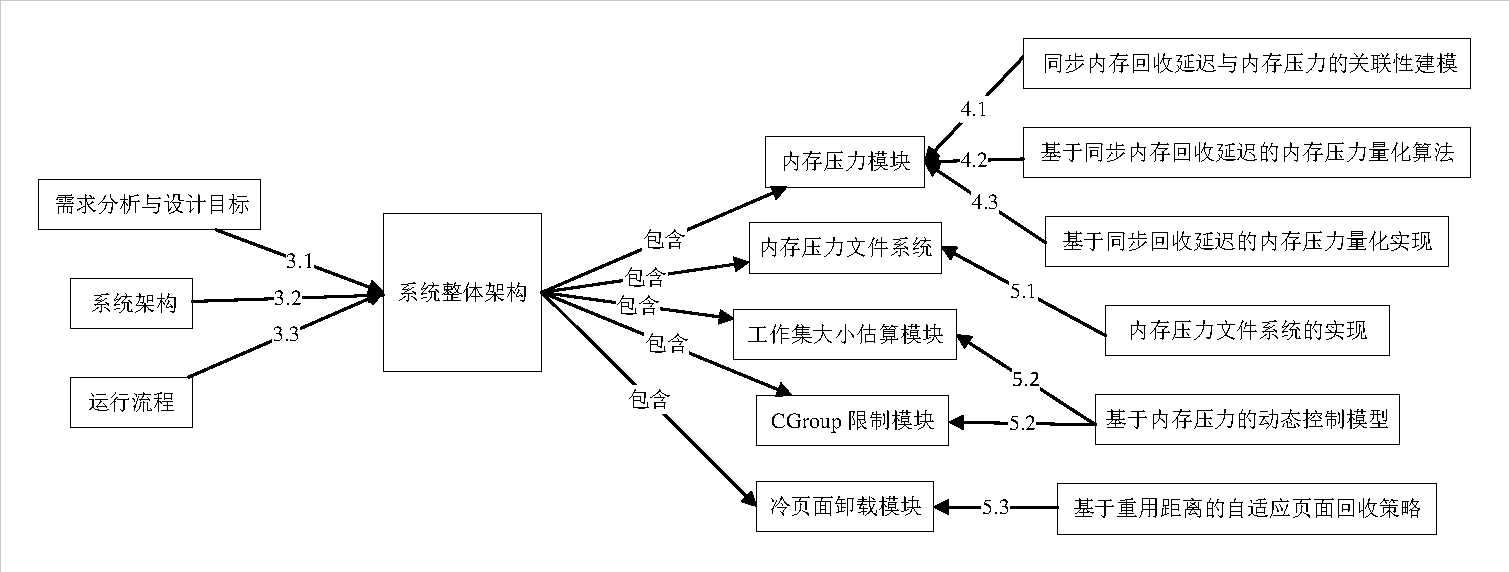
\includegraphics[width=\textwidth,keepaspectratio]{各章节研究关系.pdf}
    \caption{各章节研究关系}
    \label{各章节研究关系}
\end{figure}

本论文围绕面向异构后端的自适应主动卸载架构展开系统性研究,共分为七章。各章节的内容安排如图\ref{各章节研究关系}所示,详见下文具体说明。

第一章为绪论,主要阐述本研究的背景与意义,系统梳理了国内外分层内存技术和工作集估计算法的研究历史与现状,并明确了本论文的主要贡献与创新点。

第二章对内存管理及相关技术进行介绍,重点分析了Linux内存管理技术的核心机制,包括物理内存管理机制、虚拟内存分页机制、CGroup V2以及内存回收机制。同时,详细介绍了分层内存架构的主要技术,包括超越内存框架、NVM技术以及RDMA技术,为后续研究奠定技术基础。

第三章提出了面向异构后端的自适应主动卸载架构的总体设计方案。首先进行了需求分析并明确了设计目标,随后详细阐述了系统架构,包括内存压力模块、通信模块以及内存管理模块的功能与职责。最后,详细描述了框架的初始化过程和执行流程,阐明了各模块间的协同工作机制。

第四章重点研究了基于同步内存回收的内存压力量化算法。首先建立了同步内存回收延迟与内存压力的关联性模型,提出了基于同步内存回收延迟的内存压力量化算法,并针对多核加权聚合、时间漂移处理以及定点数优化等方面进行了深入研究。随后,详细阐述了基于生产者消费者模式的内存压力量化实现,包括工作流程、工作队列、临界区保护以及内存压力计算算法的具体实现细节。

第五章构建了基于内存压力的主动卸载框架。首先实现了内存压力文件系统,将内核中计算的内存压力指标有效暴露到用户态;其次,提出了基于内存压力的动态调控模型;最后,详细设计了基于重用距离的自适应页面回收策略,包括重用距离的近似推导、替换决策与回收策略,以及基于阴影条目的重用距离追踪内核实现方法。

第六章进行了系统的实验测试与结果分析。首先明确了实验环境与测试负载,随后对内存压力模块和文件页与匿名页均衡算法进行了有效性验证。在此基础上,设计了综合测试方案,对系统整体性能进行了全面评估,并对测试结果进行了深入分析与讨论。

第七章对全文研究内容进行了总结,分析了当前方案存在的局限性,并提出了未来研究的改进方向与展望。


